% ---------------------------------------------------------------------
\section{Plate Recognition}
\label{sec:lprnet}

\subsection{OCR baselines}

\paragraph{EasyOCR.} With $3\times$ upscaling, histogram equalisation and an
alphanumeric allow-list the output was mostly garbled: confidence was 0.06--0.46
on the first test image and 0.11--0.61 across ten test images, and the plate
\plate{KL01BM5673} came back as strings such as \plate{KLYGIBH5673}. On 218
hand-labelled scenes the exact-match rate was only 17--25\,\% in fog (light fog
25\,\%, severe fog 17\,\%) and 6--11\,\% in rain, with a character error rate of
0.45--0.74 (Figure~\ref{fig:easyocr}). EasyOCR is a general scene-text reader; it
confused \plate{1}/\plate{I} and \plate{7}/\plate{Z} and failed on small
blurred plates.

\paragraph{Other readers.} PaddleOCR could not be run to completion (an internal
inference-engine error of its Windows CPU build). The plate-specific
\emph{fastplateOCR} was clearly better and read \plate{KL01BM5673} as
\plate{KL01BM567}, 9 of 10 characters correct, but it consistently dropped
the trailing digit of 10-character Indian plates and its repeated readings of
one plate varied (Figure~\ref{fig:ocr}). This was the decision point to build a
reader for Indian plates.

\begin{figure}[t]
\centering
\begin{subfigure}[b]{0.56\textwidth}
  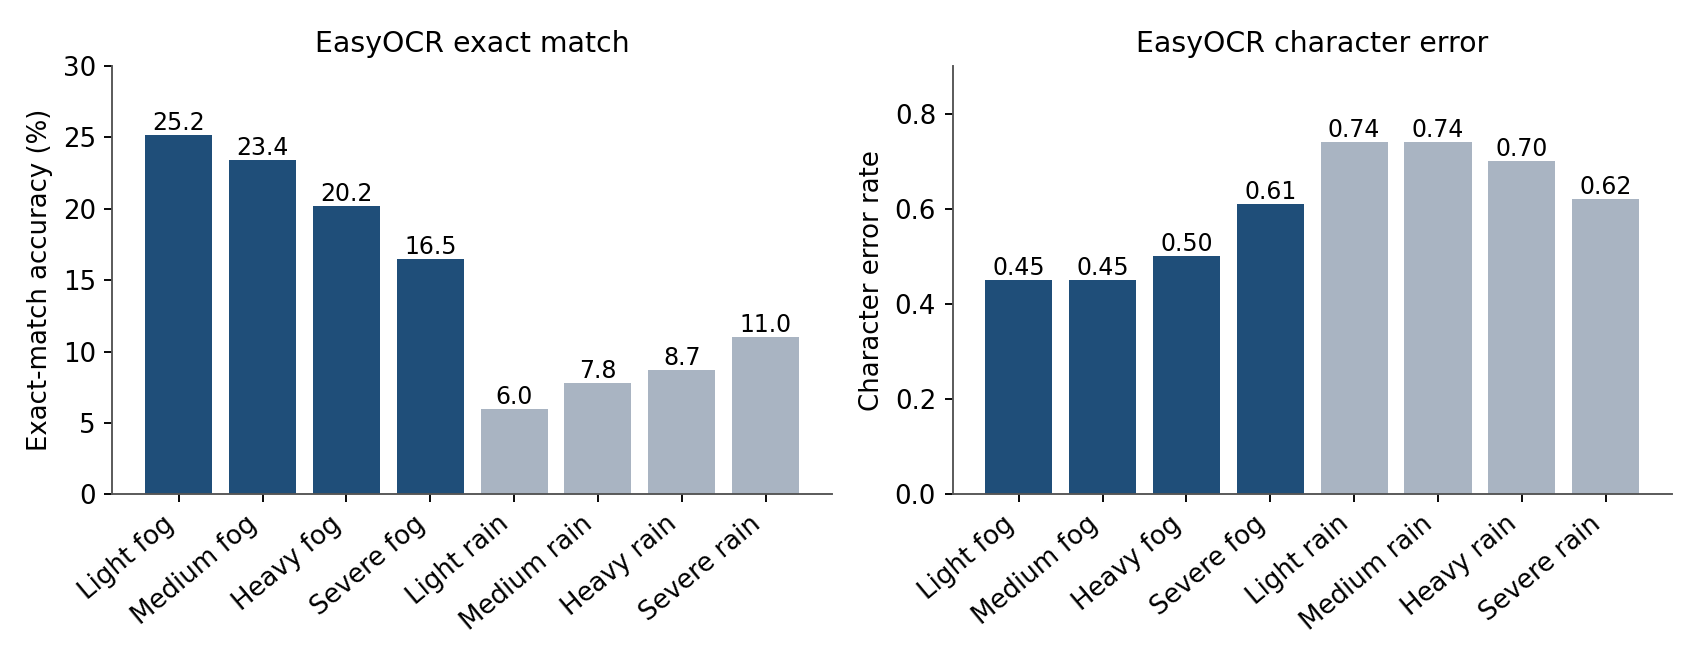
\includegraphics[width=\textwidth]{easyocr_weather.png}
  \caption{EasyOCR exact match and character error by weather.}
  \label{fig:easyocr}
\end{subfigure}\hfill
\begin{subfigure}[b]{0.40\textwidth}
  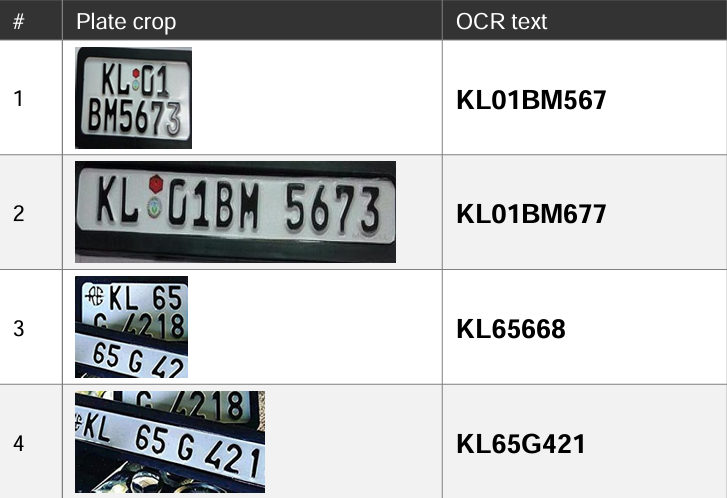
\includegraphics[width=\textwidth]{ocr_baselines.png}
  \caption{Readings of the baseline OCR engines on sample plates.}
  \label{fig:ocr}
\end{subfigure}
\caption{Baseline OCR results.}
\end{figure}

\subsection{LPRNet}

LPRNet~\cite{zherzdev2018lprnet} is a convolutional network that reads the whole
plate in one pass. The plate crop is resized to $200\times24$ pixels and the
network outputs, for each of its horizontal positions, a probability over the 36
characters A--Z and 0--9 and a CTC blank. With the CTC loss~\cite{graves2006ctc}
the training target is the plate string and no per-character boxes are needed.
Two-line plates (common on two-wheelers, autos and some cars) are flattened
into one row before reading by cutting the crop at its horizontal midline and
placing the lower half after the upper one. For crops whose aspect ratio is
ambiguous (between 1.9 and 2.6) both readings, single-line and flattened, are
made and the plate-looking, higher-confidence one is kept.

\subsection{Training in stages}

Trained from scratch on the 218 labelled scenes the network overfitted
badly: the training loss fell to 0.32 but the validation exact match stayed at
0--6\,\% with a character error rate of 0.70, because the data held only about
197 distinct plates. Pre-training on synthetic plates (30\,000 random plates per
epoch) raised the synthetic validation accuracy from 78.5\,\% to 99.5\,\%,
showing that the network was sound and that diversity of data was the limit.
Each later step added a kind of data that the earlier readers lacked
(Table~\ref{tab:lpr}):
\begin{itemize}
  \item \textbf{Fine-tuning and mixing.} Fine-tuning on the real plates gave
        34--37\,\% exact match with a character error of 0.32; mixing synthetic
        plates into the fine-tuning and adding 40\,000 images of the CCPD
        set~\cite{xu2018ccpd} lowered the character error to 0.249 (44\,\%
        exact; Figure~\ref{fig:lprcer}).
  \item \textbf{Real Indian plates.} The reader was fine-tuned on normal and
        CAPTCHA-style crops after removing about 10\,\% junk, on our own Kerala
        photographs labelled with a review page, and on the public Zenodo
        plate set (about 1\,355 pairs). With 16 Kerala plates held out as a fixed
        test, exact reads rose from a mean of 6.7 to 9.0 of 16 over three seeds.
        Because every retrain broke different plates, results are reported over
        multiple seeds and the weights of the best runs are averaged.
  \item \textbf{Degradation.} Training with shrinking to 12--30 pixels height,
        blur, motion and JPEG compression halved the character error on small
        video plates (0.50 to about 0.31).
  \item \textbf{Repeated characters.} CTC drops one of repeated characters
        (\plate{KL21AA2696} read with one \plate{A}, \plate{888} read as
        \plate{88}); synthetic plates with repeated characters raised per-frame
        exact reads on a video from 14\,\% to about 46\,\%.
  \item \textbf{Real video crops.} A review page (\code{video\_label\_review})
        turns each tracked plate in traffic videos into labelled crops from one
        typed label. Round~1 (114 plates, 4\,926 crops) raised exact plates on
        an unseen video from 19 to 22 of 27; round~2 (93 more plates, 1\,850
        crops) raised six held-out test videos from 38 to 41 of 51 plates
        (Figure~\ref{fig:realgain}). The test videos were never used for
        training.
  \item \textbf{Hard cases.} Photographs of 250 Rajasthan plates showed that
        Delhi plates with a lettered RTO code (\plate{DL3CCU5010}) had no
        layout, that \plate{Q} made up only 0.37\,\% of real characters
        and that red temporary plates had never been seen; a layout was added
        and synthetic plates with red backgrounds and \plate{Q} were generated.
        Exact reads on 62 held-out crops rose from 48 to 56, with the video
        benchmark unchanged (75 against 74--75).
\end{itemize}

\begin{table}[t]
\centering
\caption{Progress of the plate reader. CER is the character error rate.}
\label{tab:lpr}
\small
\begin{tabularx}{\textwidth}{@{}Xp{4.6cm}@{}}
\toprule
\textbf{Step} & \textbf{Result}\\
\midrule
Trained from scratch on 218 scenes & 0--6\,\% exact, CER 0.70\\
Synthetic pre-training + real fine-tune & 34--37\,\% exact, CER 0.32\\
+ CCPD and synthetic mixing & 44\,\% exact, CER 0.249\\
+ Zenodo plates (Kerala, 16 held out) & 6.7 to 9.0 of 16 exact\\
+ degradation training (small video plates) & CER 0.50 to 0.31\\
+ repeated-character synthetic plates & per-frame exact 14\,\% to 46\,\% (video)\\
+ real video crops, rounds 1 and 2 & 19 to 22 of 27; 38 to 41 of 51\\
+ Rajasthan plates, red plates, \plate{Q} & 48 to 56 of 62 (held-out crops)\\
\bottomrule
\end{tabularx}
\end{table}

\begin{figure}[t]
\centering
\begin{subfigure}[b]{0.62\textwidth}
  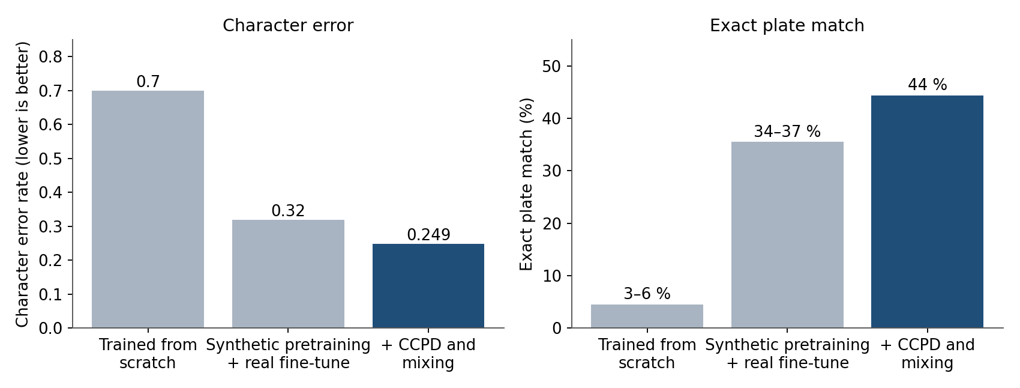
\includegraphics[width=\textwidth]{lprnet_cer_exact.png}
  \caption{Character error and exact match.}
  \label{fig:lprcer}
\end{subfigure}\hfill
\begin{subfigure}[b]{0.34\textwidth}
  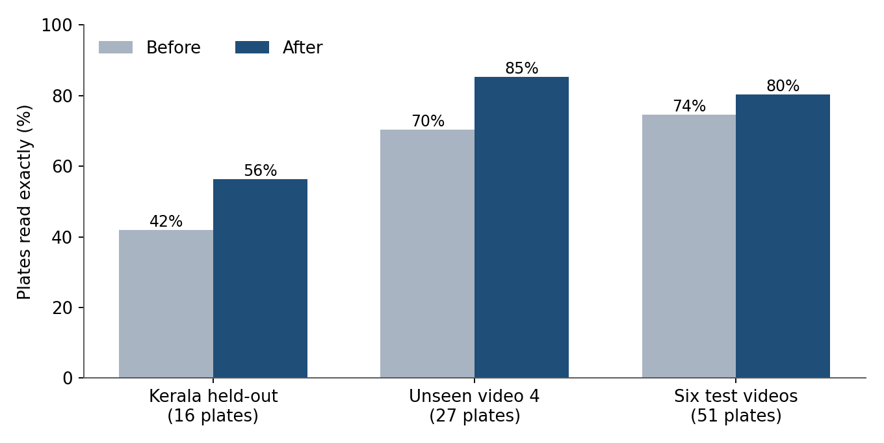
\includegraphics[width=\textwidth]{real_data_gain.png}
  \caption{Plates read before and after real-data training.}
  \label{fig:realgain}
\end{subfigure}
\caption{LPRNet results.}
\label{fig:lprresults}
\end{figure}

\subsection{Format-constrained decoding}

The raw CTC output is corrected with the structure of Indian plates. A plate is
two letters (state), two digits (district), one or two letters (series) and
four digits, \eg\ \plate{KL01AB1234}; layouts for 9-character and 10-character
plates, for the 9-character Delhi style and for Delhi plates with a lettered
RTO code are known to the decoder. Instead of replacing letters and digits
with a fixed table (\plate{O}$\rightarrow$\plate{0}), the decoder uses the
network's own per-position probabilities, restricted to the characters that the
layout allows at each slot, so that characters such as \plate{Q} that a fixed
swap would destroy are recovered. Detections that do not look like a plate
(road signs, bag logos) are hidden by default.

\subsection{Reading weather-degraded plates}

A reader trained for weather (with fog and haze applied to the training crops)
and a ``select'' view that chooses between the plain and the smoothed crop gave
the best reading of the Ponmudi photographs (47--51 of 85, against 40 for the
installed reader untouched; Section~\ref{sec:ponmudi}). The installed default
reader is the result of the real-video and Rajasthan rounds above; the
weather-trained readers are kept as separate checkpoints and are evaluated
before any replacement.

% ---------------------------------------------------------------------
\section{Tracking and Real-Time Operation}
\label{sec:realtime}

\subsection{Reading plates from video}

A first video reader detected plates in every frame, tracked each plate, read
it repeatedly and took a vote over the readings, preferring readings that match
the strict plate format. A track is called reliable when at least five reads
agree and they make up at least 4\,\% of its reads. The medoid of the readings
(the reading closest to all others) is used when no clear majority exists.

\subsection{Real-time pipeline}

The offline reader took about 10 minutes for a 45~s, 1080p clip, which is not
usable for a system that must show a plate as the vehicle passes. Profiling
showed that recognition took 30\,\% of the time, detection 27\,\%, video writing
18\,\% and the per-frame vote 15\,\% (and growing with track length). The
real-time version updates the vote incrementally over the most frequent
readings, reads each plate on every frame at first (the first ten reads) and
then every third frame, stops reading a plate once its vote is stable, runs the
detector in half precision, and skips frames when it falls behind. It processed
the 45~s clip in 44~s, about 55 frames per second at 1080p, with accuracy equal
to the offline reader (20 of 27 plates on the benchmark video;
Figure~\ref{fig:speed}). Plates that stay in view for only a few frames are
announced when they leave, if the reading is well formed (at least three agreeing
reads and 30\,\% agreement).

Reading and detection run in parallel worker processes, each with its own
detector and reader, with frames passed through shared memory and results
re-ordered into frame order; tracking and voting stay in one place so that the
output is identical to the single-process run. On 4K footage the ceiling is the
CPU decoding rate of about 27 frames per second (Table~\ref{tab:fps}).

\begin{table}[t]
\centering
\caption{Throughput in frames per second for different numbers of worker
processes (no frame skipping).}
\label{tab:fps}
\small
\begin{tabular}{@{}lcccc@{}}
\toprule
\textbf{Video} & \textbf{1 process} & \textbf{2 workers} & \textbf{4 workers} & \textbf{6 workers}\\
\midrule
1080p, 60 fps & 40.9 & 51.5 & 61.8 & 47.0\\
4K & 13.5 & 19.7 & 19.0 & 16.5\\
\bottomrule
\end{tabular}
\end{table}

\begin{figure}[t]
\centering
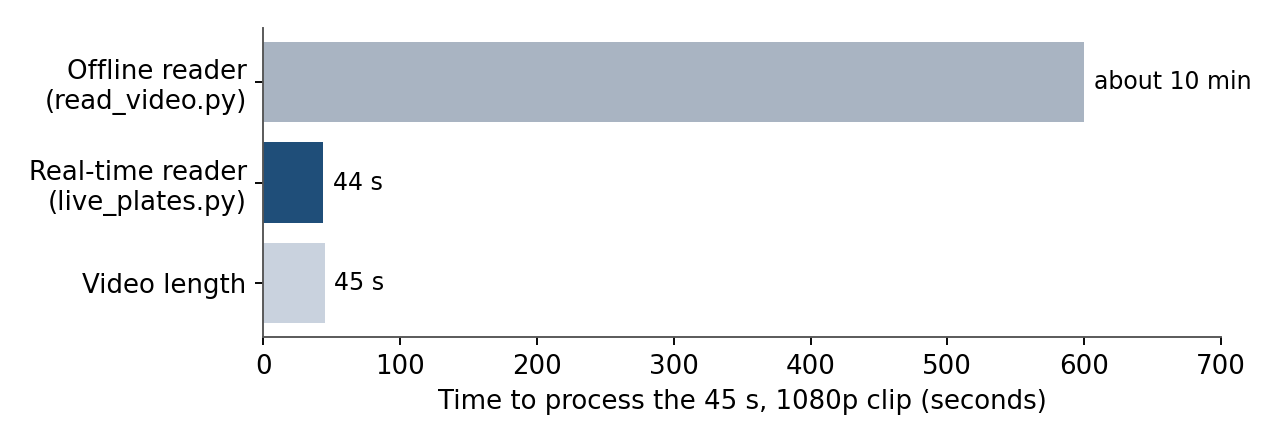
\includegraphics[width=0.75\textwidth]{offline_vs_live_time.png}
\caption{Time to process a 45~s, 1080p clip with the offline reader and the
real-time pipeline.}
\label{fig:speed}
\end{figure}

% ---------------------------------------------------------------------
\section{Tests on Unseen Traffic Videos}
\label{sec:video}

\paragraph{First test video (1.MOV, 4K).} Thirteen plates were announced. Ten of
the twelve real plates were read exactly (Table~\ref{tab:vid1}). One plate lost a
digit (\plate{KL2C6050} for \plate{KL20C6050}), one plate partly hidden by a
shadow could not be verified, and a phone-number sign on a scooter was
announced as a plate (\plate{BP20OB9200}). One yellow-plate vehicle was not
announced because the readings of its bottom-line letter split between several
characters. The live view and the announced plates are shown in
Figures~\ref{fig:live} and~\ref{fig:announced}.

\begin{figure}[t]
\centering
\begin{subfigure}[b]{0.48\textwidth}
  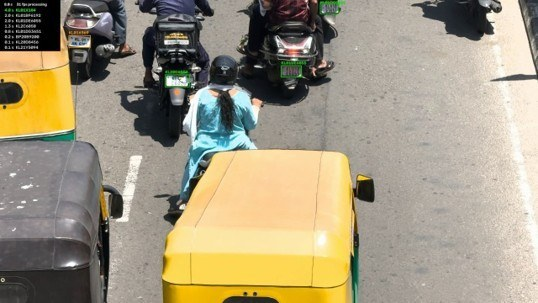
\includegraphics[width=\textwidth]{live_view_1.jpg}
\end{subfigure}\hfill
\begin{subfigure}[b]{0.48\textwidth}
  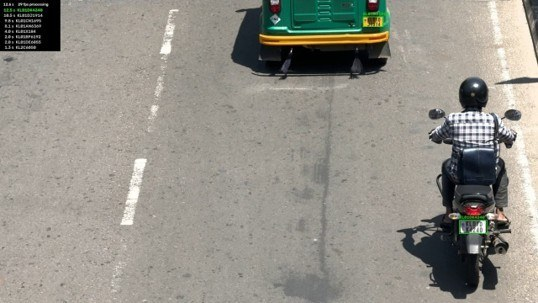
\includegraphics[width=\textwidth]{live_view_2.jpg}
\end{subfigure}
\caption{Live output: plate boxes with readings, and the list of confirmed
plates with their times at the top left; the second frame is a few seconds later.}
\label{fig:live}
\end{figure}

\begin{figure}[t]
\centering
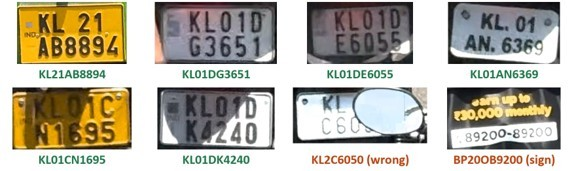
\includegraphics[width=0.8\textwidth]{announced_plates.png}
\caption{Plate crops and the readings announced: six correct, one dropped digit,
one sign read as a plate.}
\label{fig:announced}
\end{figure}

\begin{table}[t]
\centering
\caption{Results on the first test video.}
\label{tab:vid1}
\small
\begin{tabularx}{\textwidth}{@{}llX@{}}
\toprule
\textbf{Outcome} & \textbf{Plates} & \textbf{Detail}\\
\midrule
Read exactly & 10 of 12 & \plate{KL21AB8894}, \plate{KL21Y5094}, \plate{KL20D8456}, \plate{KL01DG3651}, \plate{KL01DE6055}, \plate{KL01BF6192}, \plate{KL01AN6369}, \plate{KL01CN1695}, \plate{KL01DJ1914}, \plate{KL01DK4240}\\
Wrong & 1 & \plate{KL2C6050} (true \plate{KL20C6050})\\
Not verifiable & 1 & \plate{KL01X184} (plate partly hidden by a shadow)\\
Not a plate & 1 announcement & \plate{BP20OB9200} (phone-number sign)\\
Not announced & 1 vehicle & yellow plate \plate{KL01C?7591}, bottom-line letter unclear\\
\bottomrule
\end{tabularx}
\end{table}

\paragraph{Other unseen footage.} On a 4K video from a second set (video 7) the
reader confirmed 40 plates; checked by eye, about 31 were right, 6 wrong and 3
uncertain, and about 3 real vehicles were never confirmed because their plates
were blurred or faded. Reading every frame for a plate's first ten reads and
announcing short passes on exit were added after this test to catch fast
vehicles. After the later real-video rounds the benchmark video gave 23 of 27
plates exactly.

\paragraph{Known failures.} Three equal digits in a row are still dropped
(\plate{KL01CH4448} read as \plate{KL01CH448}), series from other states are weaker,
and blurred or faded plates and signs cause misses or false plates. Plates only
22--39 pixels wide on two-wheelers and autos remain unreadable; footage of
higher resolution is the main remaining lever for them.

% ---------------------------------------------------------------------
\section{Foggy Video Pipeline}
\label{sec:foggyvideo}

The pieces of this chapter were combined into a single pipeline for foggy
video: UVMNet (GoPro-trained) followed by the physics-guided dehaze (strong,
$\gamma=1.25$, with the veil colour and exposure smoothed over time),
then the YOLOv11 detector (1280 pixels, confidence 0.25) and finally the
installed LPRNet with the ``select'' view and format correction. It was run on
four short clips filmed in fog at Ponmudi (133, 161, 144 and 237 frames at
about 29 frames per second).

Two features make the result easy to inspect. First, the annotated video
\emph{slows down} by a factor of four while a plate is detected (and for four
frames afterwards), so that the annotation can be followed. Second, a box at
the top left shows, for up to three vehicles, an enlarged crop of the plate in
the current frame, the \emph{final} reading and its votes. The final reading is
the most voted reading of that vehicle over the whole clip and is fixed from the
first frame in which the vehicle appears, so that the number does not change
from frame to frame. Raw tracks that are interrupted for at most 15 frames and
whose boxes are close are merged into one vehicle before the vote.
Figure~\ref{fig:foggyvid} shows frames of the output.

\begin{figure}[t]
\centering
\begin{subfigure}[b]{0.48\textwidth}
  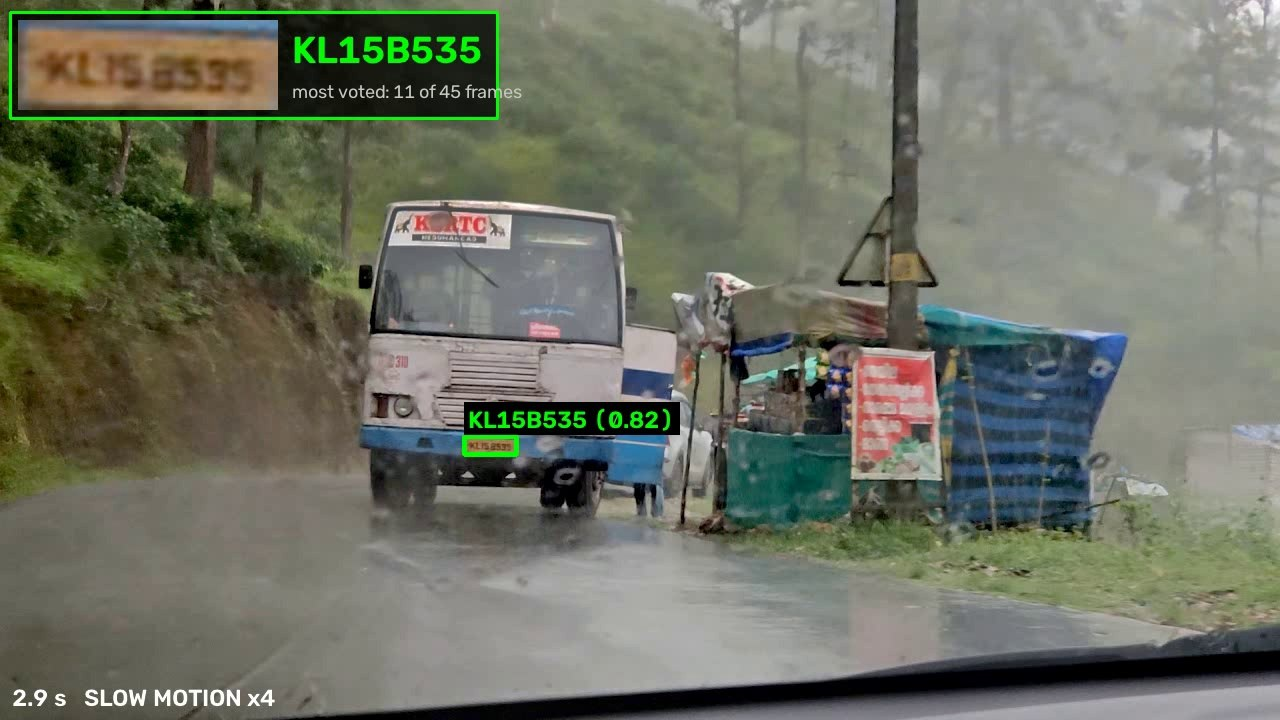
\includegraphics[width=\textwidth]{foggy_video_bus.jpg}
  \caption{A bus on the hill road.}
\end{subfigure}\hfill
\begin{subfigure}[b]{0.48\textwidth}
  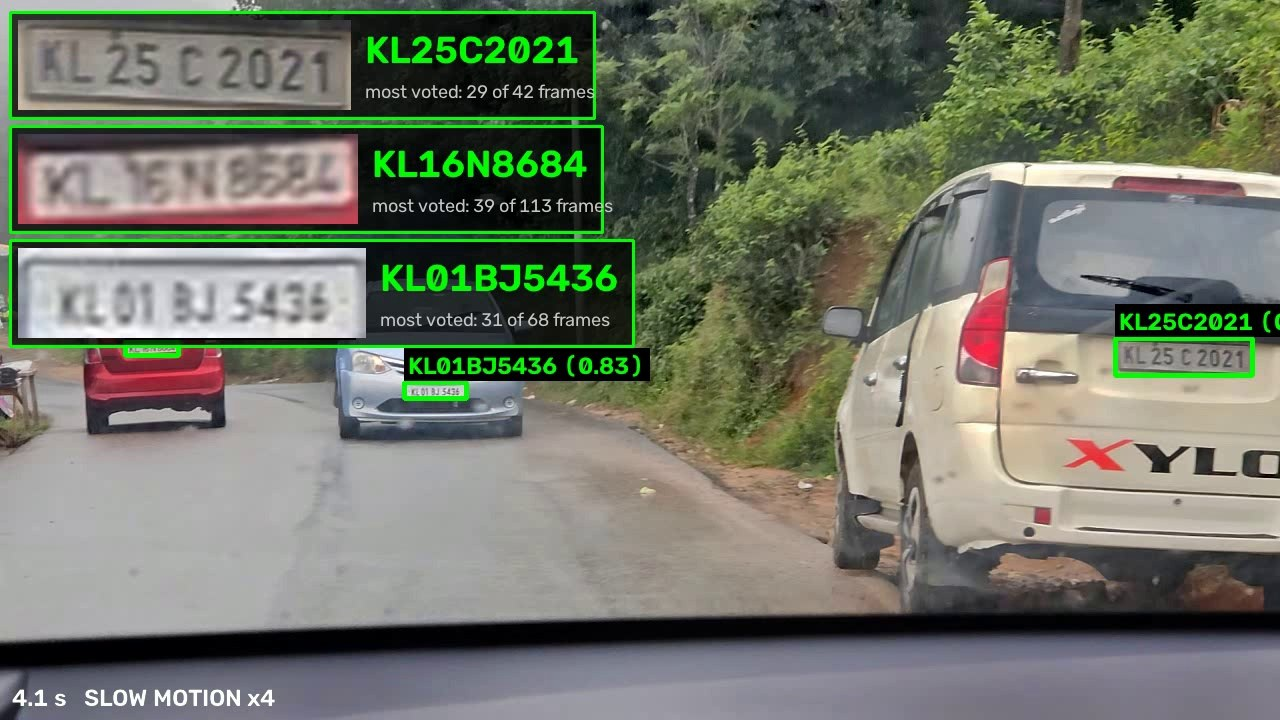
\includegraphics[width=\textwidth]{foggy_video_multi.jpg}
  \caption{Three vehicles tracked at once, each with its final reading.}
\end{subfigure}
\caption{Frames of the annotated foggy video output (slow motion $\times4$).}
\label{fig:foggyvid}
\end{figure}

\begin{figure}[t]
\centering
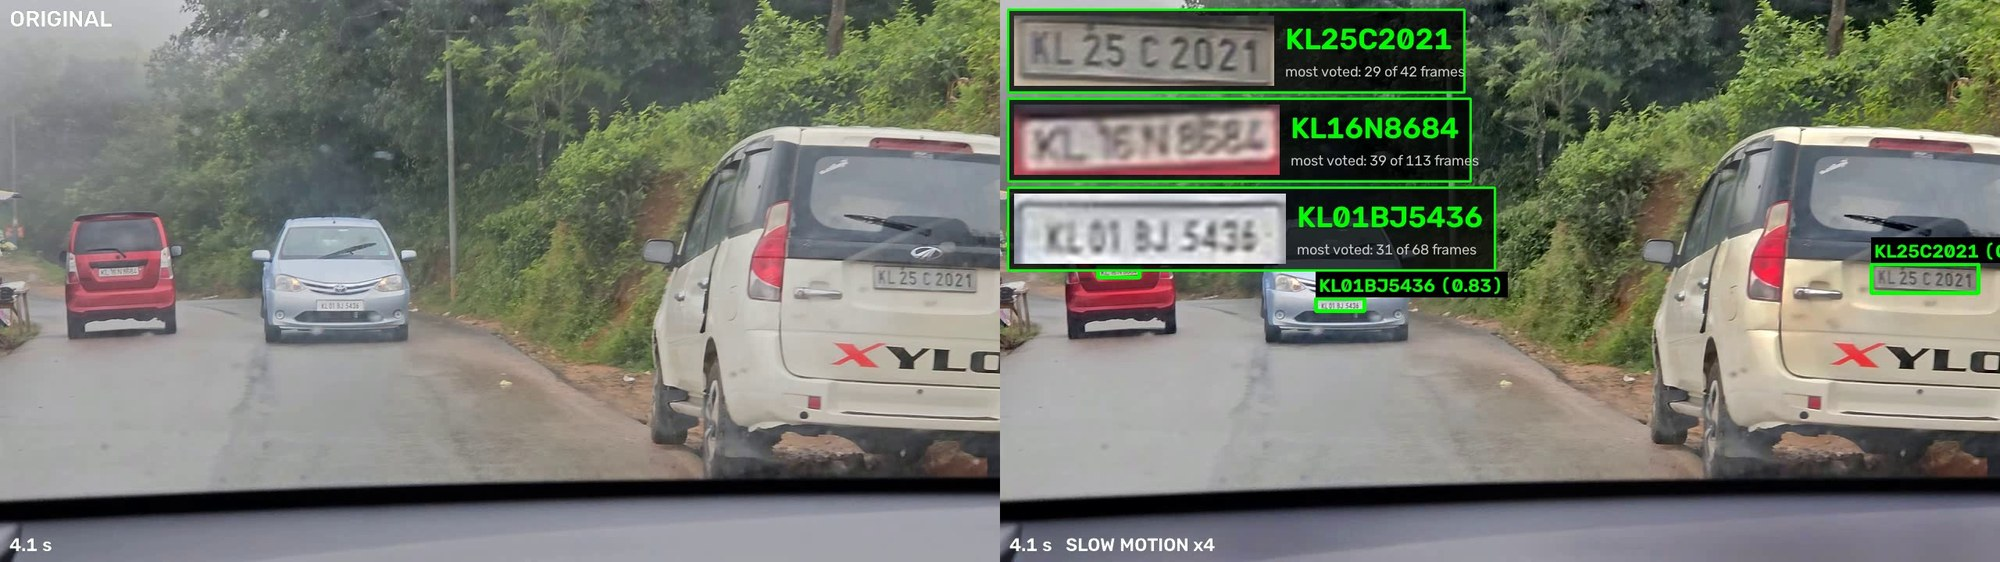
\includegraphics[width=\textwidth]{foggy_video_side.jpg}
\caption{Original (left) and dehazed, annotated (right) frame of the same
clip.}
\label{fig:foggyside}
\end{figure}

Table~\ref{tab:foggyvehicles} lists the vehicles found. The vote share is the
fraction of the vehicle's readings that agree with the final number, and is a
measure of how much to trust it. The numbers are the output of the system; the
plate crops of \plate{KL25C2021}, \plate{KL16N8684} and \plate{KL01BJ5436} agree
with the final readings by eye, whereas the readings with a vote share below
about 35\,\% (video~1, video~3) should be regarded as unconfirmed. A complete
ground-truth check of these four clips has not been done.

\begin{table}[t]
\centering
\caption{Vehicles found in the four foggy clips (final reading = most voted).}
\label{tab:foggyvehicles}
\small
\begin{tabular}{@{}llccc@{}}
\toprule
\textbf{Video} & \textbf{Final reading} & \textbf{Frames seen} & \textbf{Votes} & \textbf{Share}\\
\midrule
1  & \plate{TN10BJ0282} & 20 & 3 & 15\,\%\\
2  & \plate{KL22Q7925}  & 20 & 11 & 55\,\%\\
3  & \plate{KL15B535}   & 45 & 11 & 24\,\%\\
b1 & \plate{KL01CH7254} & 48 & 30 & 62\,\%\\
b1 & \plate{KL25C2021}  & 42 & 29 & 69\,\%\\
b1 & \plate{KL16N8684}  & 113 & 39 & 35\,\%\\
b1 & \plate{KL01BJ5436} & 68 & 31 & 46\,\%\\
b1 & \plate{KL364848}   & 2 & 1 & 50\,\%\ (unreliable)\\
\bottomrule
\end{tabular}
\end{table}

\subsection{Combining frames of the same plate}
\label{sec:fusion}

Single photographs are limited by information, but a video holds many views of
a plate. For each tracked plate up to 16 sharp crops are aligned to the
sharpest one with an affine ECC registration~\cite{evangelidis2008ecc},
upsampled by two, and combined by a weighted mean or a median; the combined
image is then read. The Ponmudi videos gave 133 plate tracks, of which nine
could be matched to verified plates, read by four readers (36 readings). A
single, widest frame gave 1 of 36 exactly right, a vote over the frames of the
track 9, and the fused image 8 (weighted mean) to 10 (median)
(Figure~\ref{fig:fusion}). The fused images are far cleaner than any single
frame, but on this small set fusion is no better than voting; for the plate
\plate{KL10BB8545} the fused image was exactly right for all six tracks
against four for the vote and one for the single frame. Combining
the frames of a vehicle, by vote or by fusion, is the clearest lever for foggy
video.

\begin{figure}[t]
\centering
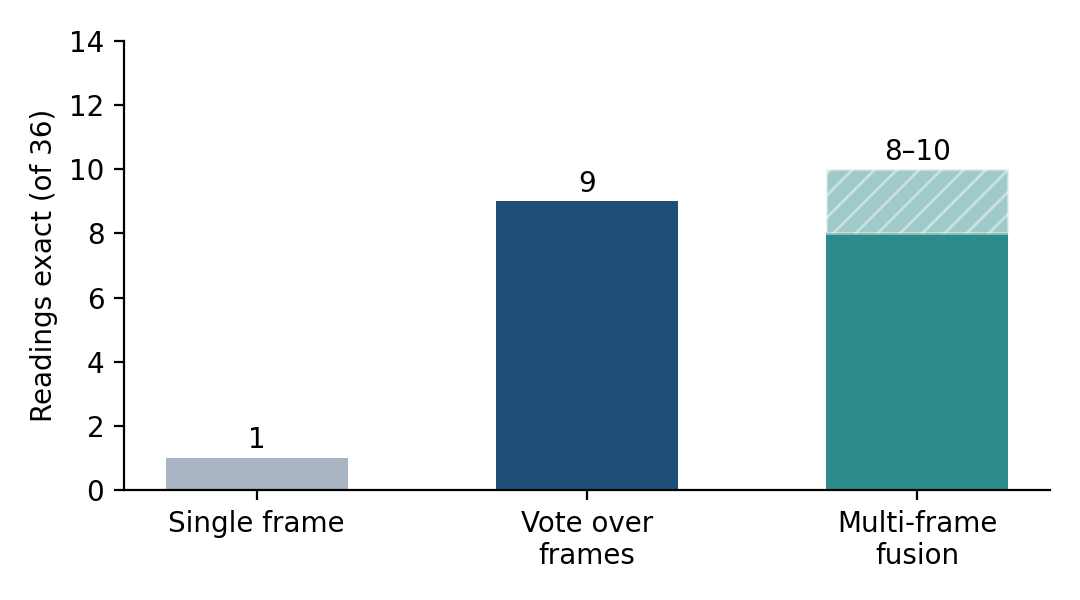
\includegraphics[width=0.6\textwidth]{video_fusion.png}
\caption{Readings exactly right (of 36) from a single frame, a vote over frames
and multi-frame fusion on the Ponmudi tracks (fusion: 8 for the mean, 10 for the
median; the hatched part shows the range).}
\label{fig:fusion}
\end{figure}

% ---------------------------------------------------------------------
\section{Browser Interface}

A browser interface (\code{plate\_app.py}) was written so that the pipeline
can be used without the command line. It lets the user pick or drop videos and
photographs (or type a path), shows the live annotated view with a list of the
confirmed plates, keeps earlier runs, and offers stop, play-back of the
annotated video and a CSV download; the number of parallel workers can be set
on the page. A second version for foggy video (\code{foggy\_plate\_app.py})
runs the UVMNet and physics-guided stages before detection and reading. Both
were tested end to end on videos by path, 4K input and photographs.

% ---------------------------------------------------------------------
\section{Summary}

Phase~1 produced a plate detector with 99.2\,\% mAP@50, a plate reader whose
exact-plate rate was raised in stages with synthetic, public and
self-labelled data, a real-time pipeline that confirms plates by voting at up
to 55 frames per second on 1080p, and fog and rain restoration models with a
physics-guided option for display. The experiments showed that the plate reader
and the combination of frames, rather than ever heavier restoration, decide how
many plates are read in bad weather.
